\problem{}
(a) The Laplacian kernel is that:
$$
\nabla^2 f = \begin{bmatrix}
    0 & 1 & 0 \\
    1 & -4 & 1 \\
    0 & 1 & 0
\end{bmatrix}
$$
The kernel is separable, and the separated kernel is:
$$
\begin{bmatrix}
    0 & 1 & 0 \\
    0 & -2 & 0 \\
    0 & 1 & 0
\end{bmatrix}
+
\begin{bmatrix}
    0 & 0 & 0 \\
    1 & -2 & 1 \\
    0 & 0 & 0
\end{bmatrix}
$$

$$\begin{bmatrix}1\\2\\1\end{bmatrix}$$
$$\begin{bmatrix}1 & -2 & 1\end{bmatrix}$$

The processed image is shown in Figure \ref{fig:p2a}.

\begin{figure}[htbp]
    \centering
	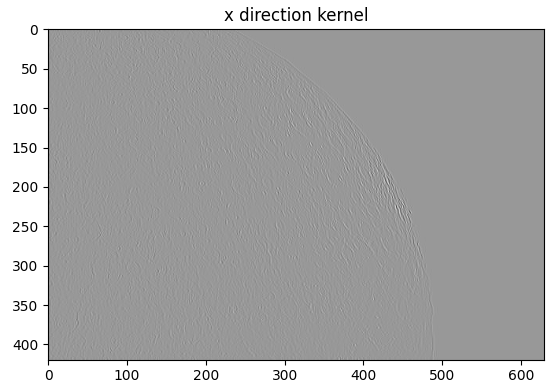
\includegraphics[width=0.48\textwidth]{../images/p2/p2a_x_direction.png}
	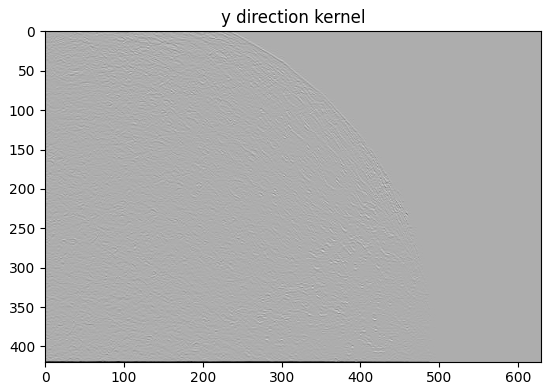
\includegraphics[width=0.48\textwidth]{../images/p2/p2a_y_direction.png}
    \caption{Separated Laplacian kernels processed image}
\label{fig:p2a}
\end{figure}


(b) Sharpened image with unseparated Laplacian kernel

1\\


The processed image is shown in Figure \ref{fig:p2b}.

\begin{figure}[htbp]
    \centering
	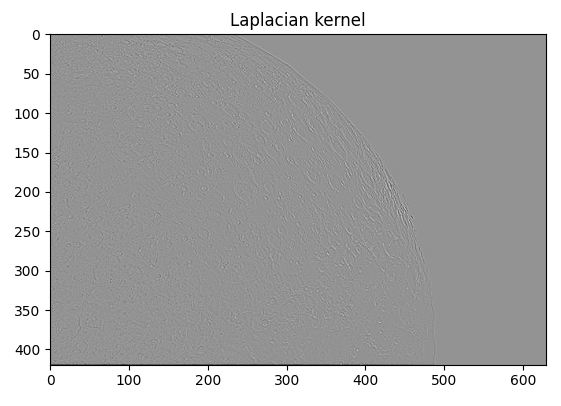
\includegraphics[width=0.48\textwidth]{../images/p2/p2b_Laplacian.png}
    \caption{Unseparated Laplacian kernels processed image}
\label{fig:p2b}
\end{figure}

(c) Sharpened image with unsharpen mask

The processed image is shown in Figure \ref{fig:p2c}.







\begin{figure}[htbp]
    \centering
	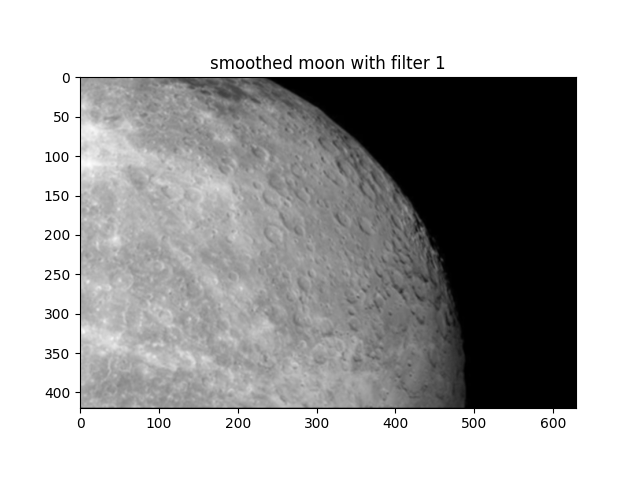
\includegraphics[width=0.48\textwidth]{../images/p2/p2c_smooth_1.png}
    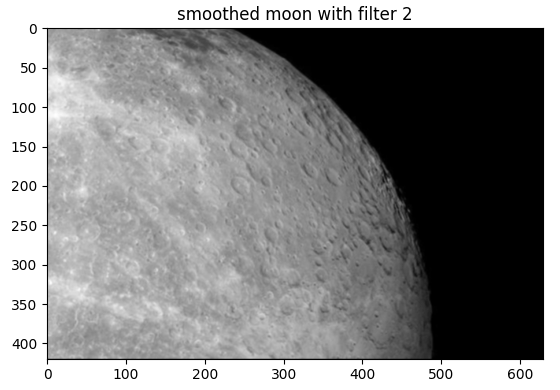
\includegraphics[width=0.48\textwidth]{../images/p2/p2c_smooth_2.png}
	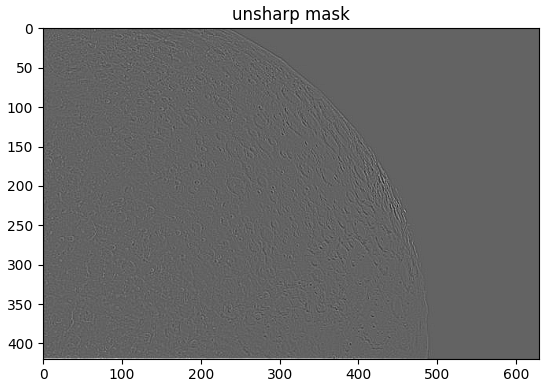
\includegraphics[width=0.48\textwidth]{../images/p2/p2c_unsharp_1.png}
	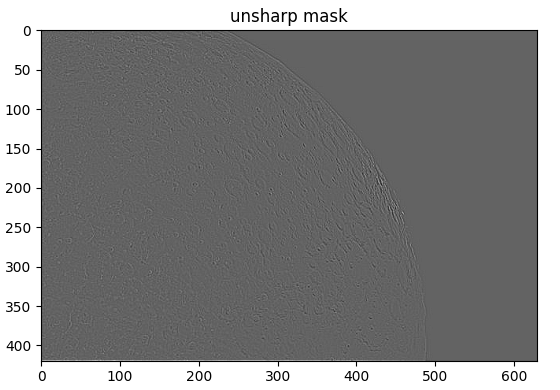
\includegraphics[width=0.48\textwidth]{../images/p2/p2c_unsharp_2.png}
	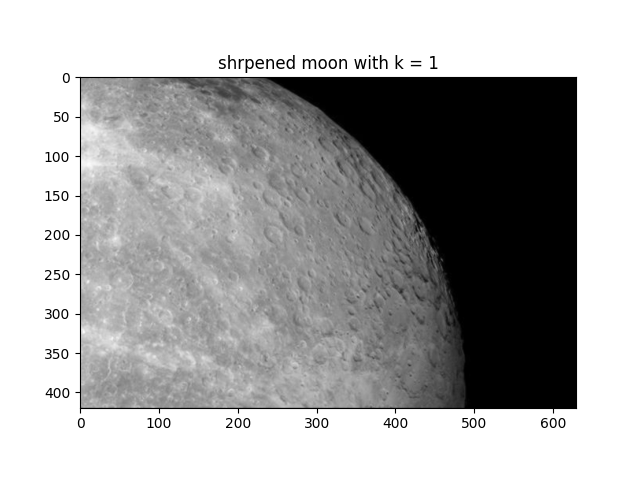
\includegraphics[width=0.48\textwidth]{../images/p2/p2c_sharpened_1_1.png}
	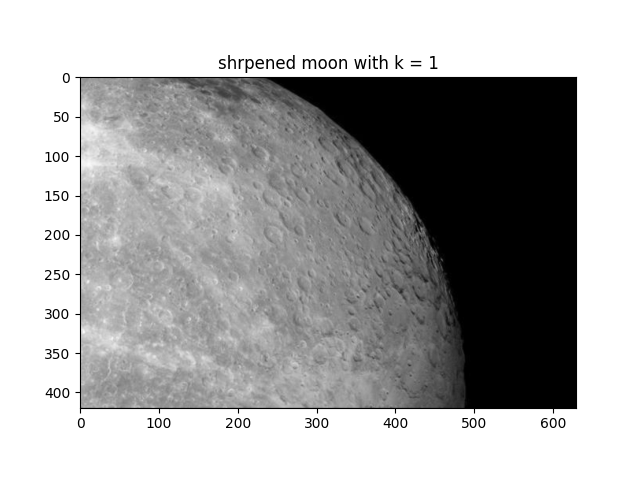
\includegraphics[width=0.48\textwidth]{../images/p2/p2c_sharpened_2_1.png}
	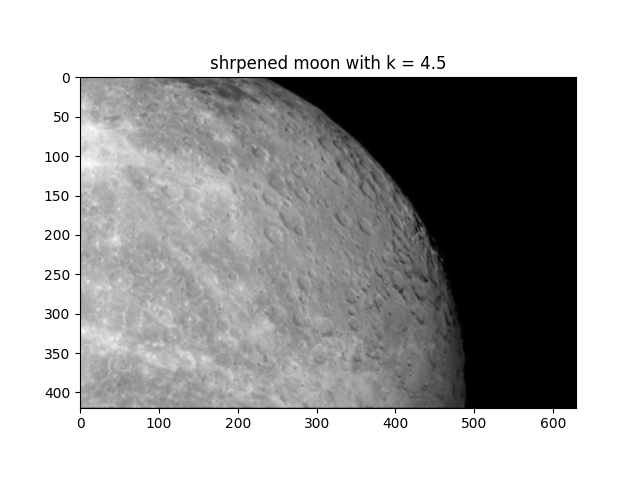
\includegraphics[width=0.48\textwidth]{../images/p2/p2c_sharpened_1_45.png}
	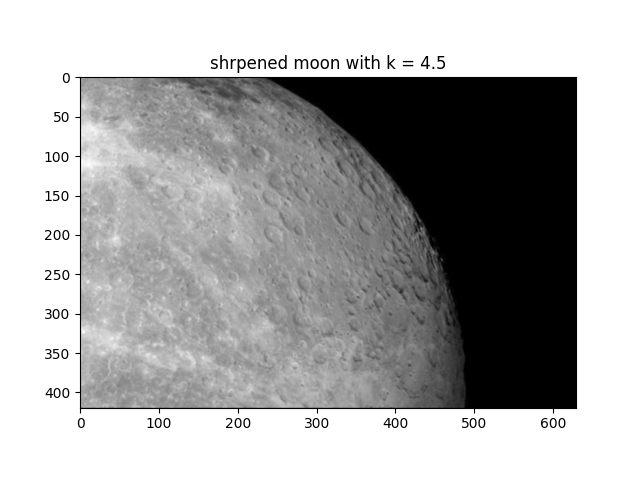
\includegraphics[width=0.48\textwidth]{../images/p2/p2c_sharpened_2_45.png}
    \caption{unsharpen mask processed image}
\label{fig:p2c}
\end{figure}

\newpage